\documentclass{article}

\setlength{\evensidemargin}{0in} \setlength{\oddsidemargin}{0in}
\setlength{\textwidth}{6.7in} \setlength{\topmargin}{-1.1in}
\setlength{\textheight}{10.5in}

\usepackage{amssymb, amsthm, amstext, amsxtra, amsmath, amsfonts, amscd }
\usepackage{graphicx, epsfig}
\usepackage{comment, color, cleveref, listings, wrapfig}

\definecolor{dkgreen}{rgb}{0,0.6,0}
\definecolor{gray}{rgb}{0.5,0.5,0.5}
\definecolor{mauve}{rgb}{0.58,0,0.82}
\definecolor{backcolour}{rgb}{0.95,0.95,0.92}

\lstdefinestyle{mystyle}{ frame=tb, backgroundcolor=\color{backcolour}, 
language=R, aboveskip=3mm, belowskip=3mm, showstringspaces=false,
columns=flexible, numbers=none, keywordstyle=\color{blue}, tabsize=3,
numberstyle=\tiny\color{gray}, commentstyle=\color{dkgreen},
stringstyle=\color{mauve}, breaklines=true, breakatwhitespace=true}
\lstset{style=mystyle}

\def\E{\mathbb{E}}
\def\pr{\mathbb{P}}

\renewcommand\baselinestretch{1.2}

\DeclareMathOperator{\sign}{sign}
\DeclareMathOperator{\supp}{supp}

\DeclareMathOperator{\Cov}{Cov}
\DeclareMathOperator{\Var}{Var}
\DeclareMathOperator{\corr}{corr}

\author{Salvador Garcia, s1655274}
\date{17 February 2017}
\title{Assgn4: Salmonella Data}
  
\begin{document}
\maketitle
\section{Description of the problem} 
  

\vspace{0.3cm}

Breslow (1984) analyses mutagenicity assay data on salmonella in which three plates have each been processed at various doses of quinoline (0,10,33,100,333,1000),  and the number of  colonies of TA98 salmonella subsequently measured.

\vspace{0.1cm}

Denote the dose by $x_i$, $i=1,\ldots,6$, and the number of colonies observed on plate $j$ at dose $x_i$ by $y_{i,j}$, $j=1,2,3$.

The theory suggests the following model for $\mu_{i} = E y_{i,j}$:
$$
\log (\mu_i) = \alpha + \beta \log(x_i + 10) + \gamma x_i, \quad \text{ with } \alpha,\beta,\gamma \in \mathbb{R}.
$$

\section{Likelihood}

The proposed model by Breslow considers the following likelihood for the $y_{i,j}$:
$$
y_{i,j} \mid \mu_i \sim Pois(\mu_i) \quad \text{ independently (given) } \mu_i ).
$$

\section{Prior}
For the prior distribution in the model, three noninformative priors will be used for $\alpha,\beta,\gamma \in \mathbb{R}$ ($N(0, 100^2)$). One for each parameter. In the first part of this report, the data for dose $x_i = 100$ will be excluded from the analysis. In the second part, the predictive distribution will be compared with the observed data for the dose $x_i = 100$. 


\section{Posterior inference}

\subsection{Converge analysis}
When running the first model (with $X_i = (0,10,33,100,333,1000)$), the autocorrelation for each of the parameters $\alpha$, $\beta$ and $\gamma$ is very strong and the chains does not look good. 

  \begin{figure}[ht!]
  \centering
  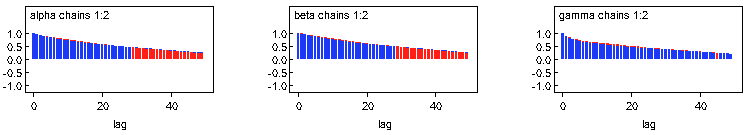
\includegraphics[width=1\textwidth]{Figures/1.png}
  \caption{Autocorrelation for the parameters $\alpha$, $\beta$ and $\gamma$.}
  \label{fig:fig1}
  \end{figure}
  
  \begin{figure}[ht!]
  \centering
  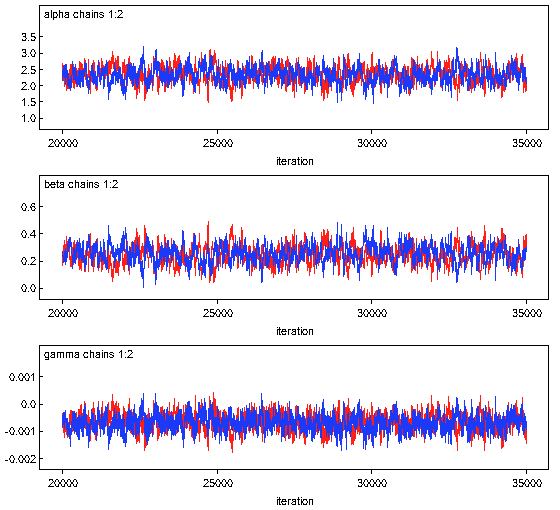
\includegraphics[width=.75\textwidth]{Figures/2.png}
  \caption{Chain for the parameters $\alpha$, $\beta$ and $\gamma$.}
  \label{fig:fig2}
  \end{figure}

This problem can be solved when thinning the chain. Due to the strong correlation, a thinning of 50 will be used. With this modification the chains look much better and the autocorrelation for the three parameters is almost gone. 

  \begin{figure}[ht!]
  \centering
  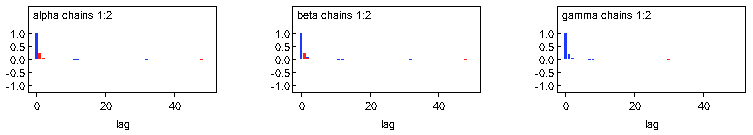
\includegraphics[width=1\textwidth]{Figures/4.png}
  \caption{Autocorrelation for parameters $\alpha$, $\beta$ and $\gamma$ with thinning of 50.}
  \label{fig:fig3}
  \end{figure}
  \begin{figure}[ht!]
  \centering
  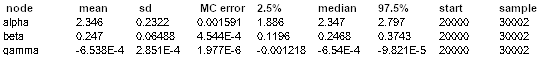
\includegraphics[width=.8\textwidth]{Figures/5.png}
  \caption{Statistics for the parameters $\alpha$, $\beta$ and $\gamma$ with thinning of 50.}
  \label{fig:fig5}
  \end{figure}
  \begin{figure}[ht!]
  \centering
  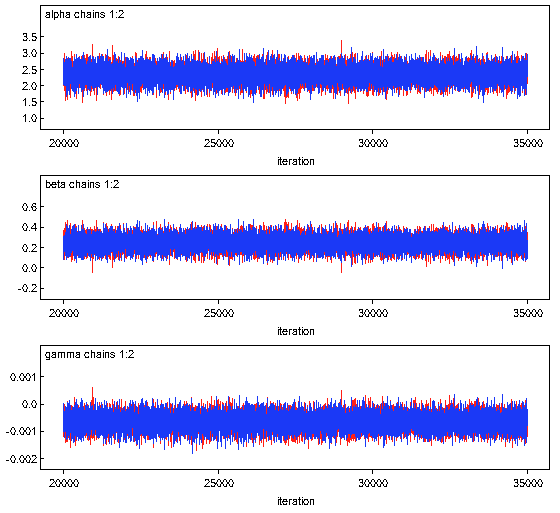
\includegraphics[width=.75\textwidth]{Figures/3.png}
  \caption{Chain for the parameters $\alpha$, $\beta$ and $\gamma$ with thinning of 50.}
  \label{fig:fig4}
  \end{figure}


\newpage  
\subsection{Residuals analysis}
The Poisson distribution only uses one parameter $\lambda$ (in this example, $\mu_i$ for $i = 1,...,6$). And also, it have the property that:

\begin{equation}
\begin{aligned}
E(y_{i,j}| \mu_i) = \mu_i \\
V(y_{i,j}| \mu_i) = \mu_i
\end{aligned}
\end{equation}

with $\mu_i$ the fitted parameter from our model. Then the standarised residuals can be expressed as $\frac{y_{i,j}-\mu_i}{\sqrt{mu_i}}$ with $i$ the dose and $y$ the number of colonies.

\newpage
\begin{lstlisting}[frame=single]
model {
  for (i in 1:5) {
    for (j in 1:3) {
      y[i,j]    ~ dpois(mu[i])}
    log(mu[i]) <- alpha + beta*log(x[i] + 10) + gamma*x[i]}
# priors
  alpha         ~ dnorm(0, 0.0001)
  beta          ~ dnorm(0, 0.0001)
  gamma         ~ dnorm(0, 0.0001)
# residuals 
   
  for (i in 1:5) {
    for (j in 1:3) {
  # add pearson (standardised) residuals for each observation y[i,j]
			stres[i,j]<-(y[i,j]-mu[i])/sqrt(mu[i])
	#	  p[i,j] <- phi(stres[i,j])
		
  # deviance for the ith element
     DS[i,j] <-  2*(mu[i]-y[i,j] - y[i,j]*(log(mu[i]) -log(y[i,j]) ) )
     sign[i,j] <- 2*step(y[i,j]-mu[i])-1 
  # deviance residual  
    res.dev[i,j] <- sign[i,j]*sqrt(DS[i,j])
    }
  }     
}
\end{lstlisting}

\subsection{Residual analysis}

In this section the boxplots of the residuals will be made. Each box in the plot represent the distribution of the residuals corresponding to $(i,j)$ (again, $i$ is the dose, and $j$ is the plate). From a quick analysis of the \cref{fig:fig6} and \cref{fig:fig7} is important to say that the residuals corresponding to the plate 1: (1,1), (2,1), (3,1), (4,1) and (5,1) almost  all are negative. On the other hand, the residuals corresponding to the plate 3: (1,3), (2,3), (3,3), (4,3) and (5,3) are almost always positive. This could mean some kind of preordering (for example, the plate 3 is the plate with more number the colonies).  Now, analysing (i,1), (i,2) and (i,3) for each $i$, it is common that in the mean the residuals are centered in zero. This is because in general, the boxplot (i,3) is the positive residuals, (i,1) in the negative and (i,2) with center in 0. The same idea applies to the deviance residuals. About the outliers, almost all the residuals are between -2 and 2, but there are some (for example in the plate (5,3) and (5,1)) where the whiskers are in values near 4.

  \begin{figure}[ht!]
  \centering
  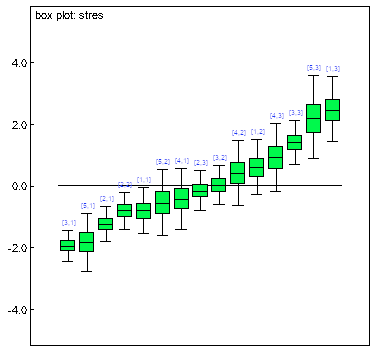
\includegraphics[width=.45\textwidth]{Figures/6.png}
  \caption{Boxplot of the standarised residuals ordered by rank.}
  \label{fig:fig6}
  \end{figure}
  
  \begin{figure}[ht!]
  \centering
  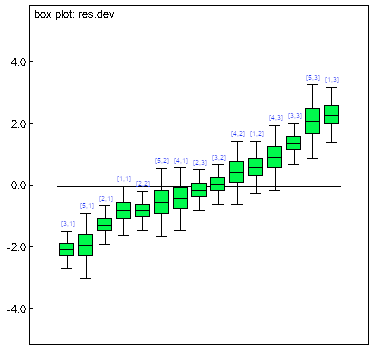
\includegraphics[width=.45\textwidth]{Figures/7.png}
  \caption{Boxplot of the deviance residuals ordered by rank.}
  \label{fig:fig7}
  \end{figure}

\newpage
\subsection{Model Fit}
For this part of the report, the model fit for each one of the plates will be analyzed \cref{fig:fig8}, \cref{fig:fig8.1}, \cref{fig:fig8.2}:

  \begin{figure}[ht!]
  \centering
  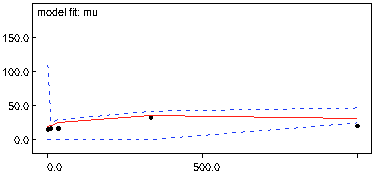
\includegraphics[width=.6\textwidth]{Figures/8_1.png}
  \caption{Model fit for plate 1}
  \label{fig:fig8}
  \end{figure}
  \begin{figure}[ht!]
  \centering
  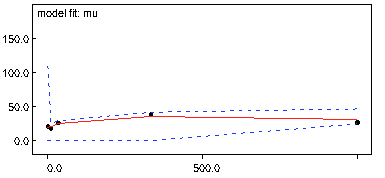
\includegraphics[width=.6\textwidth]{Figures/8_2.png}
  \caption{Model fit for plate 2}
  \label{fig:fig8.1}
  \end{figure}  
    \begin{figure}[ht!]
  \centering
  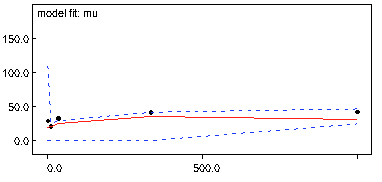
\includegraphics[width=.6\textwidth]{Figures/8_3.png}
  \caption{Model fit for plate 3}
  \label{fig:fig8.2}
  \end{figure}  

With these three plots, the idea presented in the last section (residuals) is corrobored. In the plate 1, the model prediction is larger than the original y(i,1); in the plate 2, the model prediction is close to the original y(i,2); and in the last plate (3) the prediction is smaller than the original y(i,3). About the outliers, similar conclusions from the residuals analysis will be given: For the plate 1 when x = 1000 (y(5,1)) it seems that the number of colonies observed is lower than the 95\% intervals. In addition to this outlier, the plate 3 when x = 33 (y(3,3)) seems to be outside the 95\% interval.

\newpage
\section{Predictions}

Now, we are going to obtain the predictions when x = 100. The density of the predictive distribution of $y.pred$ is presented in the \cref{fig:fig9}. The stats for this variable are in \cref{fig:fig11}

  \begin{figure}[ht!]
  \centering
  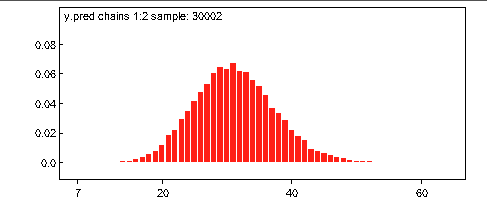
\includegraphics[width=.7\textwidth]{Figures/9.png}
  \caption{Density of the predictive distribution of $y.pred$}
  \label{fig:fig9}
  \end{figure}  
  
  \begin{figure}[ht!]
  \centering
  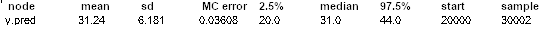
\includegraphics[width=.7\textwidth]{Figures/11.png}
  \caption{Statistics for the predictive distribution of $y.pred$}
  \label{fig:fig11}
  \end{figure}  


The observed number of colonies for this $x = 100$ is (27, 41, 60). Then, from the \cref{fig:fig9} can be see that the values of 27 and 41 are common values in this distribution, but the value 60 seems to be not very common. In fact, the 95\% credibility interval is from 20 to 44. Now, lets use the p-values p[1], p[2] and p[3] to adress the same question.


  \begin{figure}[ht!]
  \centering
  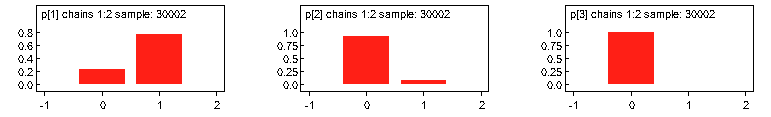
\includegraphics[width=.7\textwidth]{Figures/10.png}
  \caption{Density of p[1], p[2] and p[3]}
  \label{fig:fig10}
  \end{figure}  

  \begin{figure}[ht!]
  \centering
  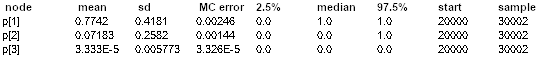
\includegraphics[width=.7\textwidth]{Figures/12.png}
  \caption{Statistics for p[1], p[2] and p[3]}
  \label{fig:fig12}
  \end{figure}  
As thinked, the p-value of p[3] is very close to 0, then for this value the prediction it is not close. p[2] and p[1] are not too close to 1 or 0: .071 and .77. In fact, they lay in the interval (.05, .95).


As an overall conclusion, for this experiment two of the three predictions are inside the confidence intervals. Although the last prediction is not in this interval, it has been shown that the plate 3 contains the original values are much bigger than in the other two plattes. 

A possible improvement to this model is to fit one model (or a variable that thakes into account this difference) for each type of plate. Another option is to try to find the variable that is making this difference. For example, maybe all the plates 1 are in total obscurity and the plates 3 recieve more sun ligth. One possible modification can be to add the total number of hours of sunlight received by the plate. I think that in general for the data that is included in this problem is a good model. But it can be improved.

If we consider the hypothesis $\gamma = 0$, taking into account the MC-error for this parameter, we can see that the MC error is approx 1.5\% of the posterior sd of the parameter gamma. So this a good number of MC-error. On the other hand, the credibility interval of this parameter is (-.001218, -.00009821) that is very close to zero, but does NOT include the 0. With a 95\% test, the hypothesis $\gamma = 0$ will be rejected.


\end{document}
  